\documentclass[14pt]{article}

\usepackage[russian]{babel}
\usepackage[utf8]{inputenc}
\usepackage{amsmath,amssymb}
\usepackage{parskip}
\usepackage{caption}
\usepackage{textcomp}
\usepackage{gensymb}
\usepackage[dvips]{graphicx}
\usepackage{wrapfig}
\usepackage{color}
\usepackage{setspace}
%\usepackage{hyperref}
\usepackage{epstopdf}

\oddsidemargin=0 cm
\evensidemargin=0 cm
\textwidth=170 mm
\textheight=230 mm
\topmargin=0 cm
\voffset= -2cm
\pagenumbering{false}
\newlength{\varheight}
\setlength{\varheight}{3.1cm}
\setlength{\parindent}{0cm}
\spacing{1.1}
\parskip=2mm
\clubpenalty=10000
\widowpenalty=10000
\captionsetup[figure]{labelformat=empty}

\begin{document}

\begin{center}
\Large{\textbf{Метод изображений}}

\textbf{15.04.2017}
\end{center}
\vspace{5mm}

{\large{Изображения в плоскости}}
\vspace{3mm}

1. Точечный заряд $q$ находится на расстоянии $d$ от бесконечной проводящей плоскости. Найдите:

а) силу и энергию взаимодействия заряда и плоскости,

б) полный заряд, наведенный на плоскости,

в$^*$) поверхностную плотность наведенного заряда в зависимости от расстояния до оси симметрии системы.

\begin{wrapfigure}{r}{70pt}
\begin{center}
\vspace{-4mm}
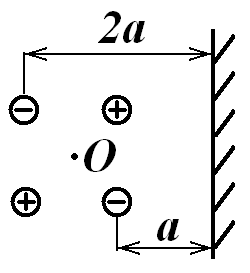
\includegraphics[scale=0.6]{images1.png}
\vspace{-1.5mm}
\caption{\hspace{-2.5mm}К задаче 2б}
\end{center}
\end{wrapfigure}

2. а) Некоторый точечный заряд в течение длительного времени удерживается на фиксированном расстоянии от бесконечной незаряженной плоскости с очень малой проводимостью. Потом заряд быстро удаляют от плоскости на расстояние, вдвое большее начального, и удерживают его в новом положении. Какое количество теплоты выделится после этого в проводящей плоскости, если известно, что за время удаления точечного заряда была выполнена работа $A=36$ мкДж?

\begin{wrapfigure}{r}{130pt}
\begin{center}
\vspace{-5mm}
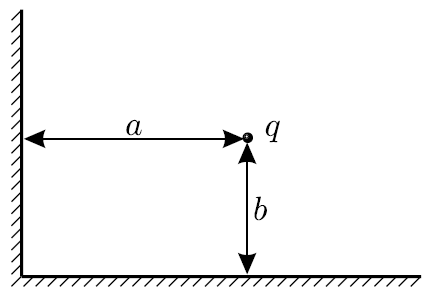
\includegraphics[scale=0.4]{images2.png}
\vspace{-6mm}
\caption{\hspace{-2.5mm}К задаче 3}
\end{center}
\vspace{-6mm}
\end{wrapfigure}

б) Квадратную рамку, в углах которой расположены заряды $+q$, $-q$, $+q$, $-q$, сначала в течение длительного времени удерживают в фиксированном положении от бесконечной незаряженной плоскости с очень малой проводимостью (рис), а потом быстро поворачивают на 90\textdegree \,вокруг оси, проходящей через центр квадрата перпендикулярно плоскости рисунка. Какое количество тепла выделится после этого в проводящей плоскости, если известно, что при повороте рамки была выполнена работа $A=36$~мкДж?

3. Две проводящие полуплоскости образуют прямой двугранный угол. Точечный заряд $q$ находится на расстояниях $a$ и $b$ от граней этого угла (см. рис). Найдите полную энергию взаимодействия зарядов в этой системе.

4. Длинный прямой проводник с током $I$ находится на высоте $d$ над бесконечной сверхпроводящей плоскостью.

а) Какой ток является изображением данного? Найдите силу и характер (притяжение/отталкивание) их взаимодействия.

б) Найдите распределение магнитного поля $\vec{B}$ в системе.

в$^*$) Определите модуль и направление линейной плотности наведенных токов в зависимости от расстояния до прямой, лежащей посередине между током и его изображением.

5$^*$. Две бесконечные проводящие плоскости параллельны и удалены друг от друга на расстояние $2l$. Посередине между ними находится точечный заряд $q$.

а) Найдите координаты и знаки зарядов всех изображений. Покажите, что заряд $q$ находится в равновесии.

б) Пусть заряд сместился в сторону одной из плоскостей на расстояние $x\ll l$. Найдите модуль и направление силы, действующей на заряд со стороны плоскостей. Будет ли исходное равновесие устойчивым?

Подсказка: $\sum\limits_{k=0}^\infty \dfrac{1}{(2k+1)^3}\approx 1.05$, можете считать значение этой суммы известным.

\vspace{5mm}
{\large{Изображения в сфере: IPhO 2010.1}}
\vspace{3mm}

{\large{Изображения в цилиндре}}
\vspace{3mm}

6. Длинный прямой проводник с током $I$ расположен параллельно оси длинного сверхпроводящего цилиндра радиуса $R$, расстояние между осью цилиндра и проводником $d$. Какой ток является изображением данного? Найдите силу и характер (притяжение/отталкивание) их взаимодействия.

\end{document} 